\section{Auswertung}
\label{sec:Auswertung}
\subsection{Mitlere Freie Weglänge}
Zerst wird die in der \autoref{sec:Theorie} erwähnte Mittlere Freie Weglänge  der lektronen bestimmt, die die Elektronen 
in dem Quecksilbergas zurücklegen, bis es zu einem Stoß kommt. Daz werden die Temperaturen bei denen Messungen von uns durchgeführt wurden 
in \autoref{eqn:...} eingesetzt und in \autoref{tab:10} Aufgelistet.
\begin{table}[H]
  \centering
  \caption{Mittlere Freie Weglängen.}
  \label{tab:10}
  \begin{tblr}{
      colspec = {S S },
      row{1} = {guard, mode=math},}
         \toprule
         T/\, \unit{\kelvin} &\overline{\omega}/ \unit{\meter} \\
         \midrule
          296.15&\num{0.063e3}\\
          419.15&\num{7.02e-5}\\
          436.15&\num{3.75e-5}\\
          448.15&\num{2.42e-5}\\
          \bottomrule
  \end{tblr}
\end{table}
Es ist erkennbar, dass Mehr stöße passieren, je höher die Temperatur ist. bei temperaturen im Bereich 
von $400\unit{\kelvin}$ bis $500 \unit{\kelvin}$ ist das verhältnis der Mittleren freien Weglänge zu dem 
Abstand von Kathode zu Anode von $a = 1\unit{\centi\meter} $sehr gering, was den Frank Herz Versuch ermöglicht.

\subsection{Kontaktpotential}
In diesem Teil des Versuchs geht es darum das Kontaktpotential zu berechnen. 
in den Abbildungen \autoref{fig:10} sowie \autoref{fig:11} sind die Strom-Gegenspannungs Messkurven
abgebildet, welche mit einem x-y Schreiber aufgezeichnet wurden. Einmal bei einer Temperatur von 296.15\unit{\kelvin}
und einmal bei 419.15\unit{\kelvin}
\begin{figure}[H]
  \centering
  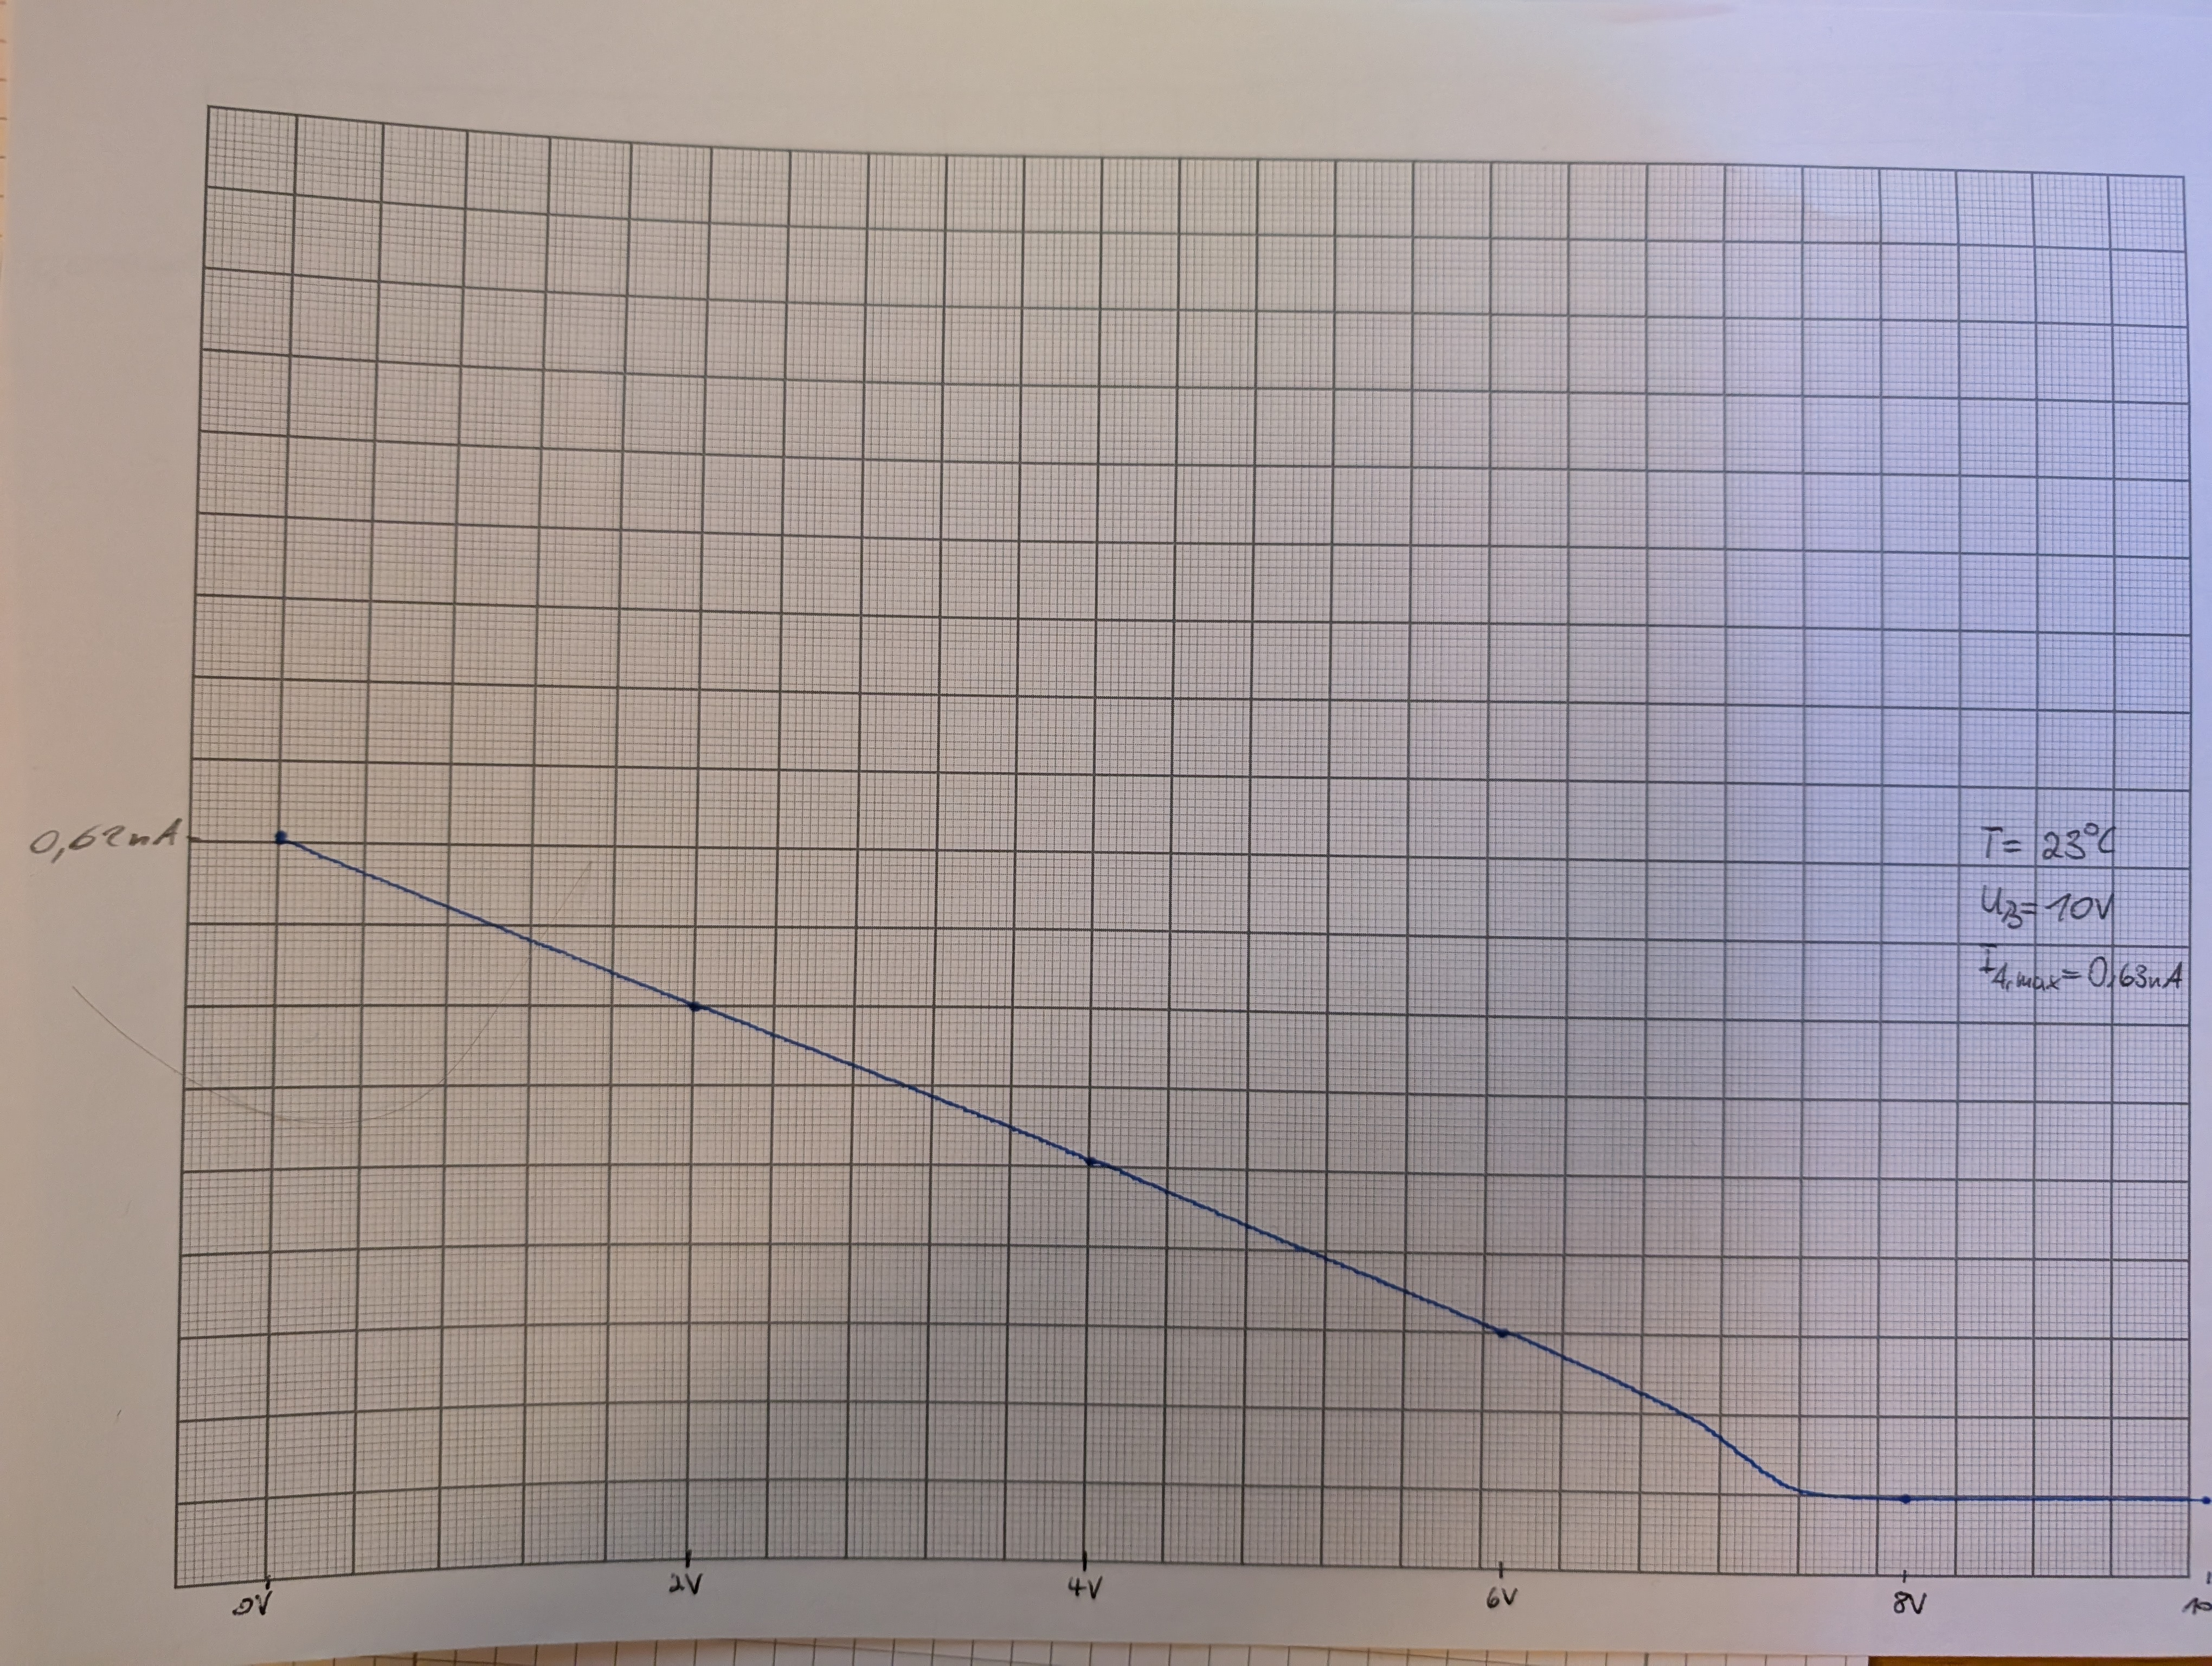
\includegraphics[width=\linewidth]{Bilder/1.jpg}
  \caption{Strom-Spannungs Kurve bei 296.15\unit{\kelvin}}
  \label{fig:10}
\end{figure}

\begin{figure}[H]
  \centering
  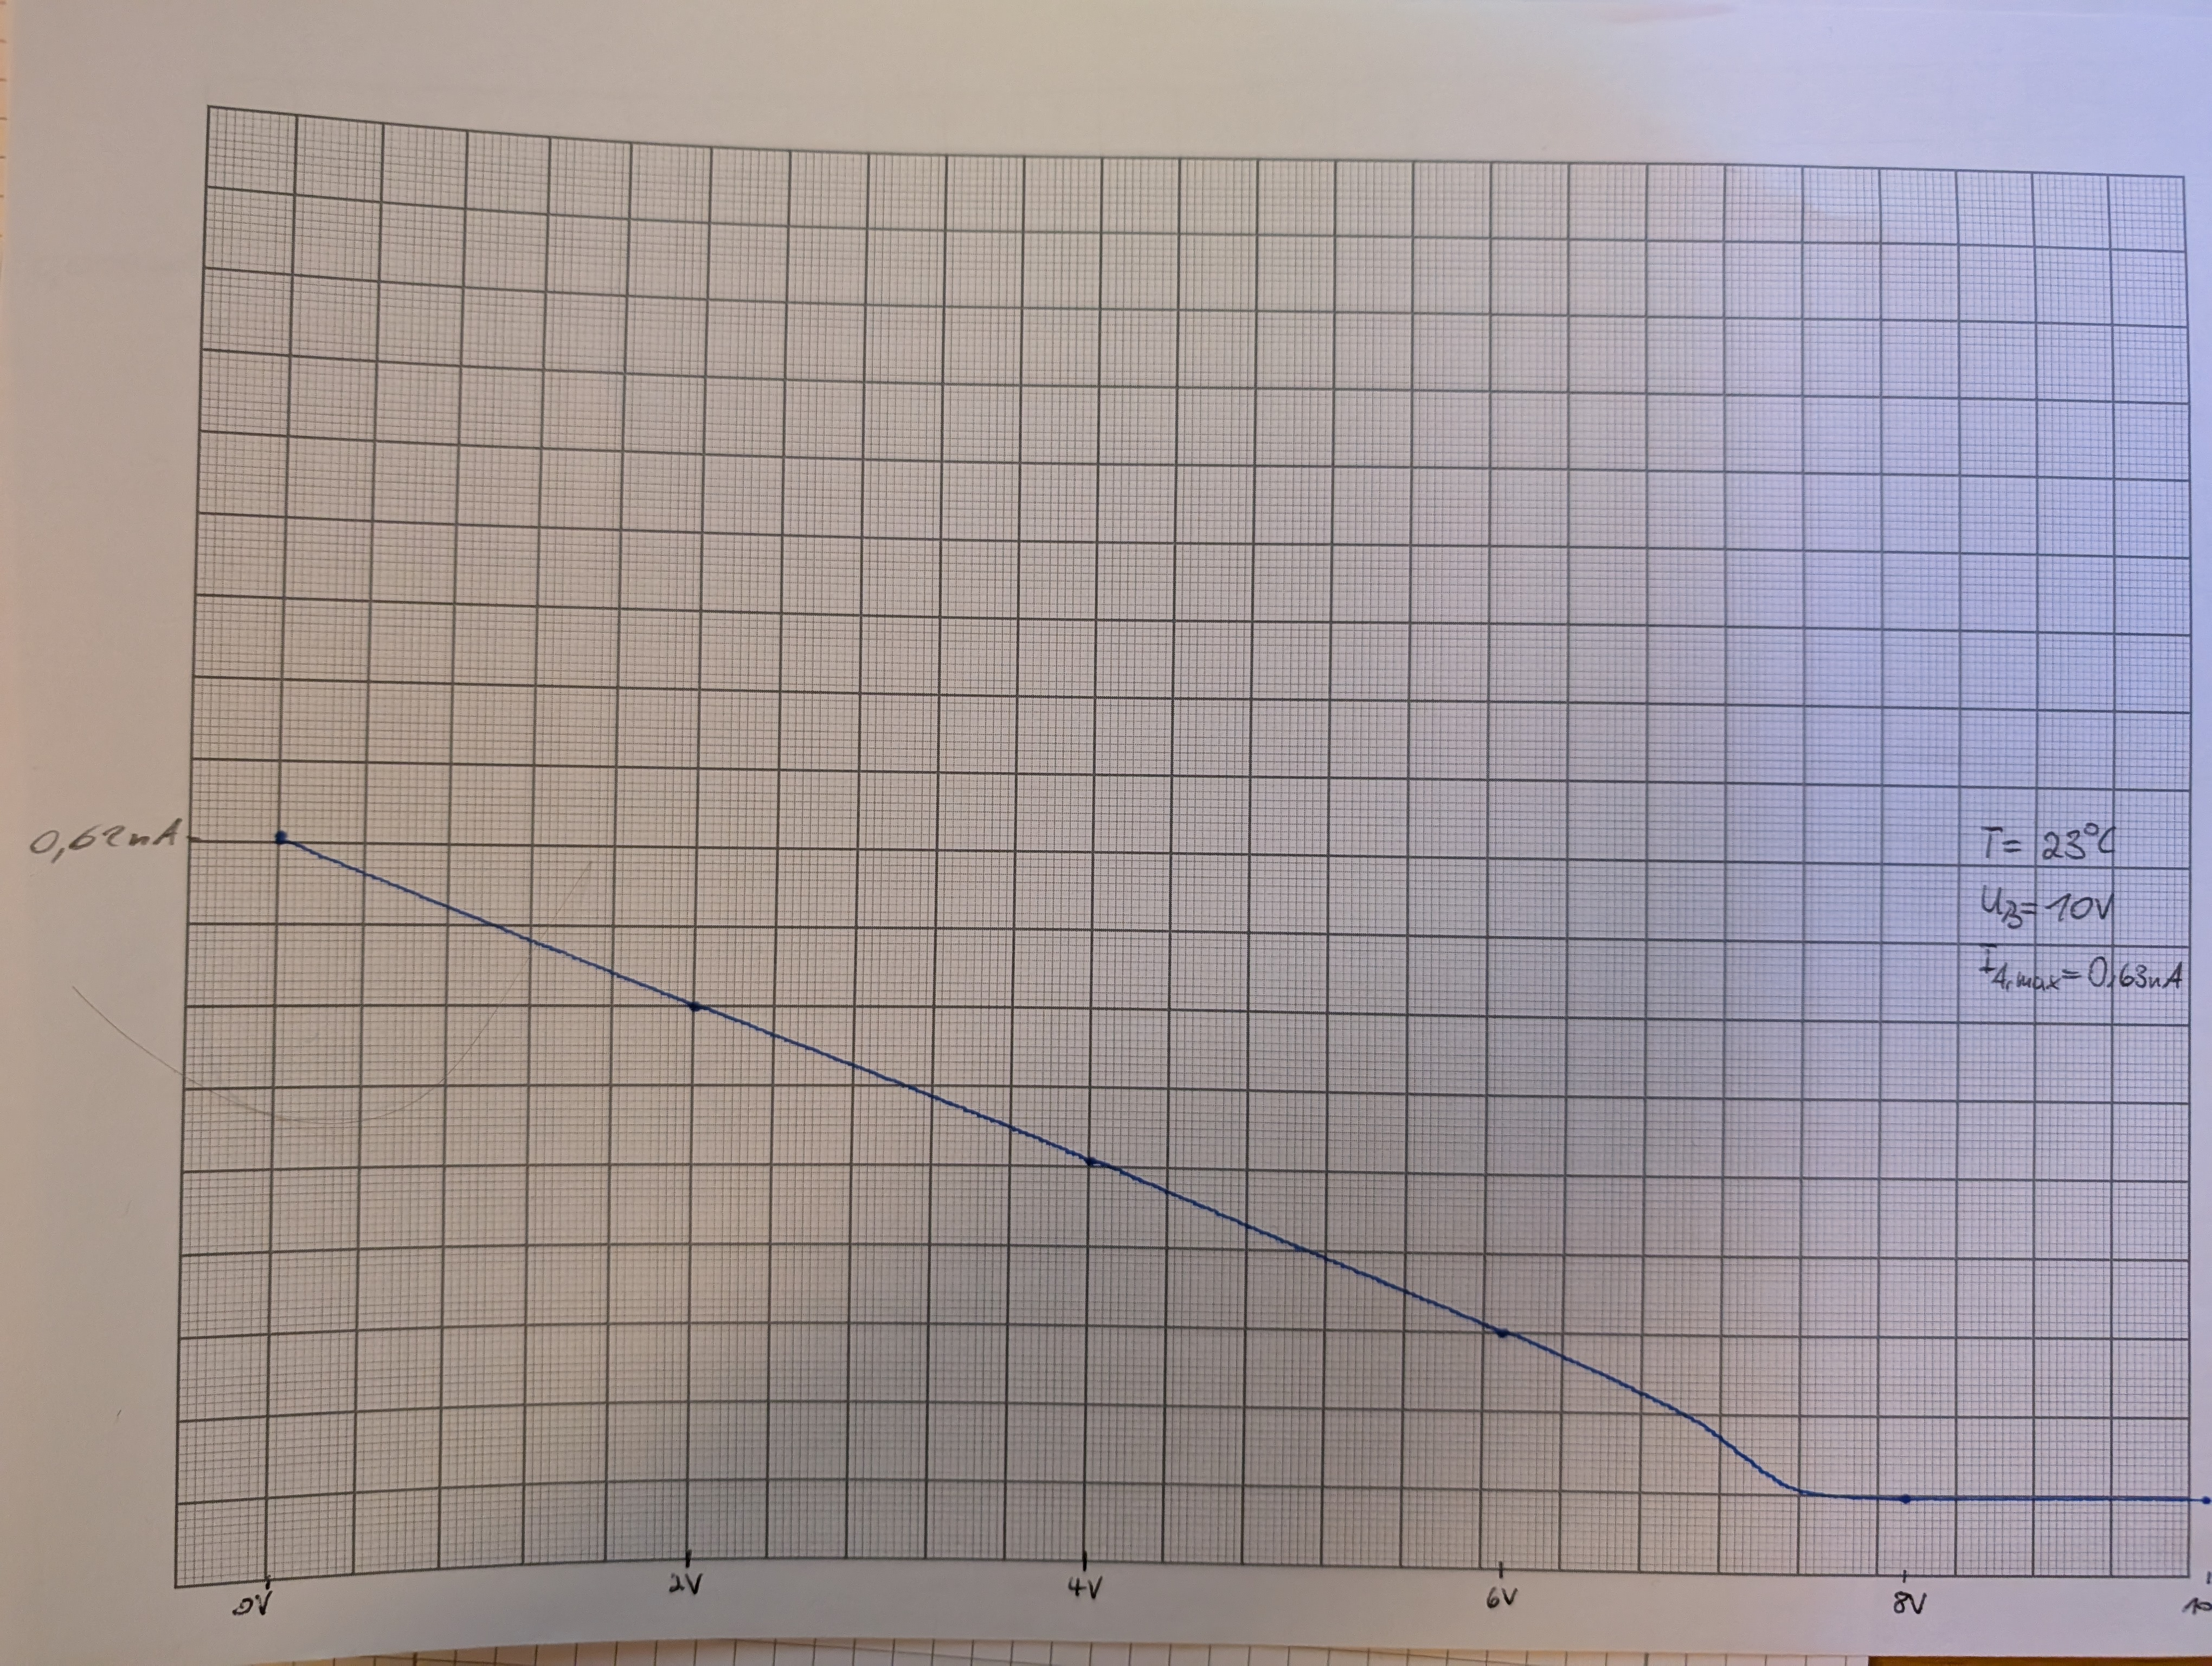
\includegraphics[width=\linewidth]{Bilder/1.jpg}
  \caption{Strom-Spannungs Kurve bei 419.15\unit{\kelvin}}
  \label{fig:11}
\end{figure}

\noindent Aus diesen Graphischen Daten muss der Differenzenquotient für einige Werte gebildet werden, 
um auf den Spannungspunkt mit der größten Steigung, also den Wendepunkt zu schließen. Daraus lässt sich dann 
nach \autoref{eqn:...} das Kontaktpotential berechnen.

\noindent In \autoref{tab:11} sind die händisch ermittelten Differenzenquotienten einiger Messpunkte für 
beide Tempoeraturen aufgeführt. Außerdem sind sie in \autoref{fig:12} und \autoref{fig:13} Graphisch dargestellt.
\begin{table}[H]
  \centering
  \caption{Differentiation der Messdaten.}
  \label{tab:11}
  \begin{tblr}{
      colspec = {S S },
      row{1} = {guard, mode=math},}
         \toprule
         T/\, \unit{\kelvin} &\overline{\omega}/ \unit{\meter} \\
         \midrule
          296.15&\num{0.063e3}\\
          419.15&\num{7.02e-5}\\
          436.15&\num{3.75e-5}\\
          448.15&\num{2.42e-5}\\
          \bottomrule
  \end{tblr}
\end{table}
\begin{figure}
  \centering
  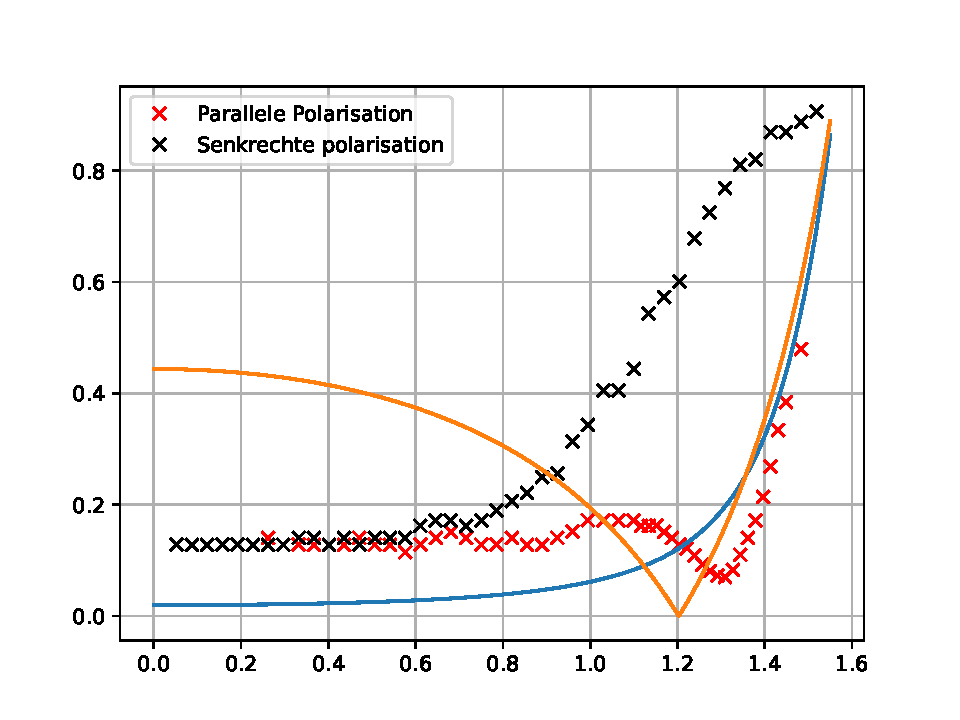
\includegraphics[width=\linewidth]{build/plot.pdf}
  \caption{Steigung der Kurve bei 296.15\unit{\kelvin}}
  \label{fig:12}
\end{figure}



\begin{figure}
  \centering
  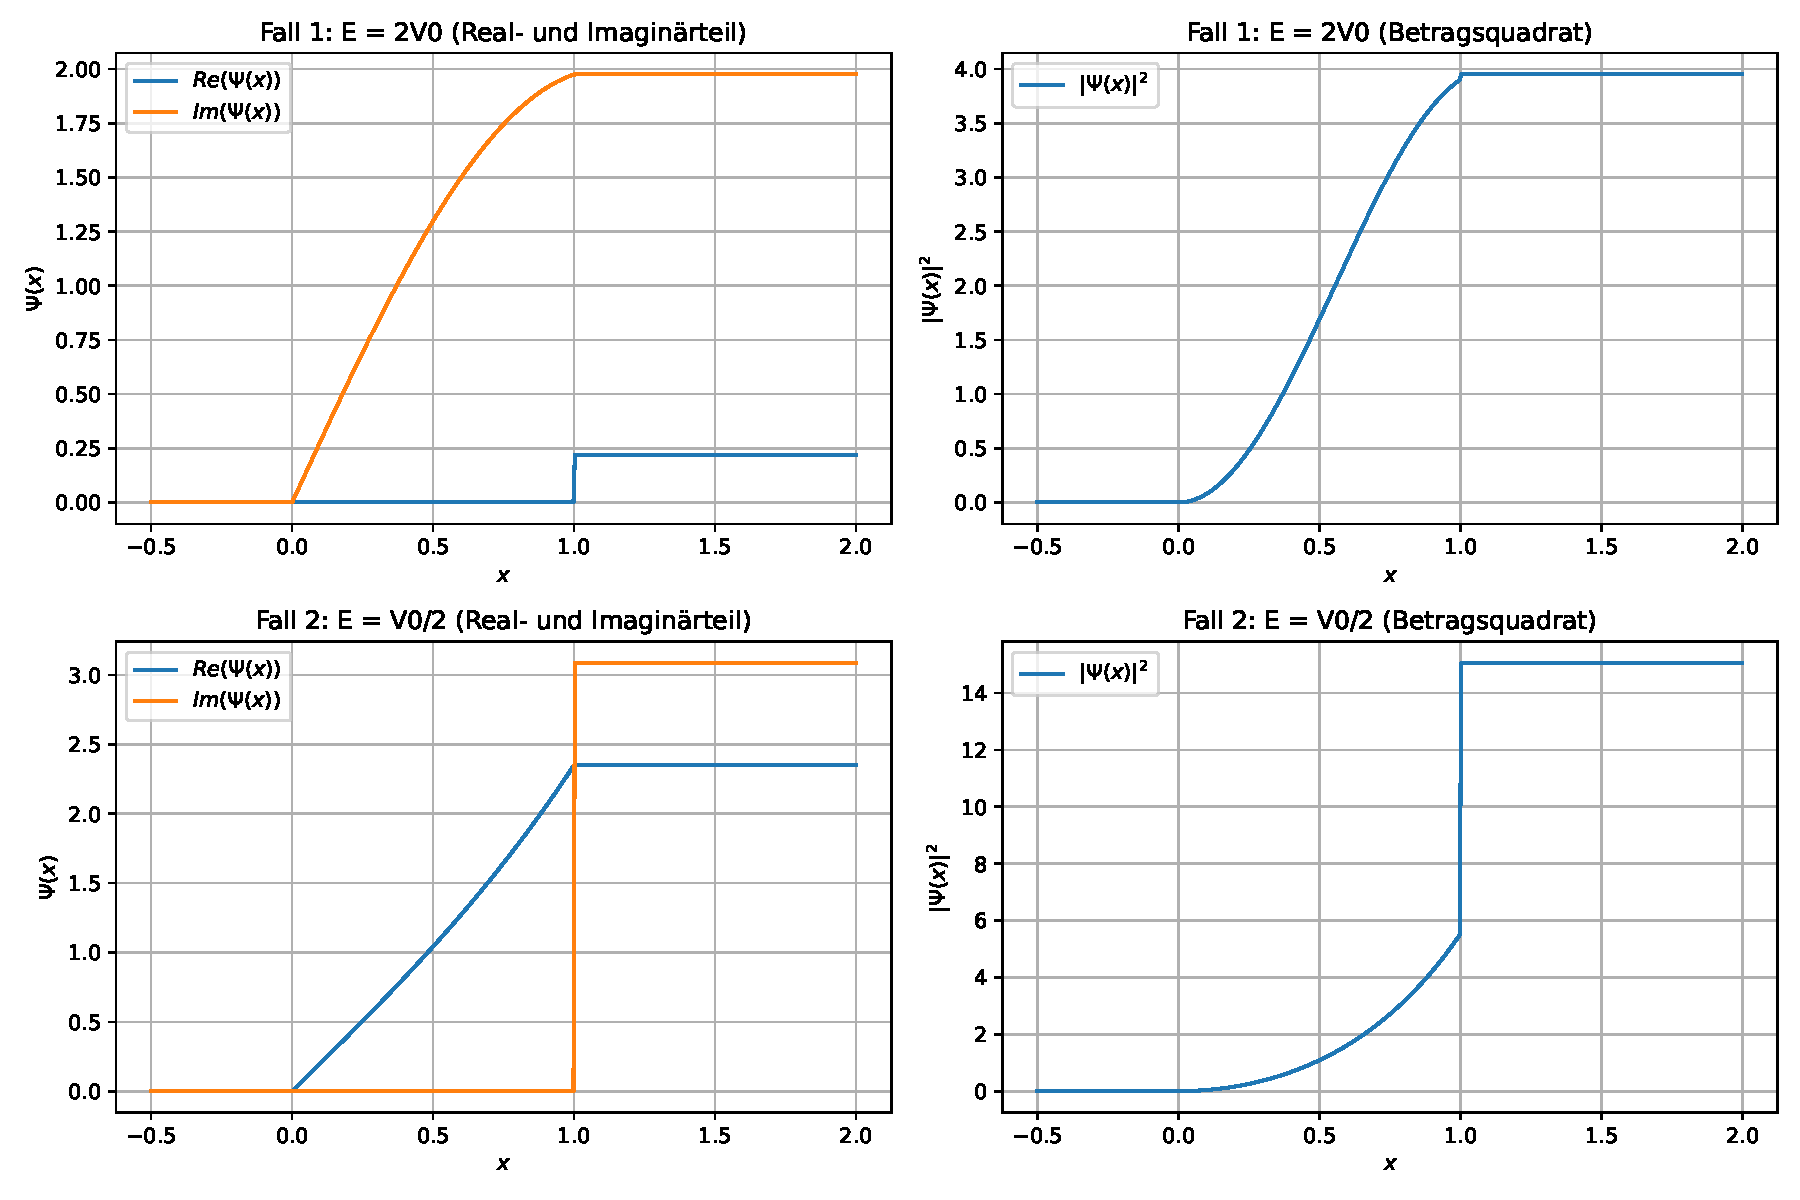
\includegraphics[width=\linewidth]{build/plot2.pdf}
  \caption{Steigung der Kurve bei 419.15\unit{\kelvin}}
  \label{fig:13}
\end{figure}

